% \PassOptionsToPackage{table}{xcolor}
\documentclass[11pt]{beamer}
\usepackage[utf8]{inputenc}
\usepackage[english]{babel}
\usepackage{amsmath}
\usepackage{amsfonts}
\usepackage{amssymb}
\usepackage{graphicx}
\usepackage{tikz}
\usepackage{algorithm}
\usepackage{algorithmic}
\usepackage{silence,lmodern}
\usepackage{csquotes}
\usepackage[backend=bibtex, bibencoding=ascii, style=authoryear, doi=false, isbn=false,url=false, uniquename=init, giveninits=true]{biblatex}
\usepackage{multimedia}
\usepackage{dirtytalk}
\usepackage{pgfplotstable,booktabs,longtable}
\WarningFilter{biblatex}{Patching footnotes failed}

% \mode<presentation>
% {
    \usetheme[hideothersubsections]{PaloAlto}
    % \usecolortheme{beaver}
% }
\usetikzlibrary{calc,trees,positioning,arrows,chains,shapes.geometric,
decorations.pathreplacing,decorations.pathmorphing,
shapes,matrix,shapes.symbols,plotmarks,decorations.markings,
shadows,shapes.geometric,arrows}

\setbeamercolor{logo}{bg=white}  %controls the color of the logo area
\setbeamerfont{footnote}{size=\tiny}

% \addbibresource{library.bib}

\makeatletter
\setlength{\beamer@headheight}{.9cm}
\makeatother

\author{S M Al Mahi}
\title[ECEN-5283 Computer Vision]{Project 3. \\ Texture Classification}
\setbeamercovered{transparent} 
\setbeamertemplate{navigation symbols}{}


\logo{
\includegraphics[width=1cm]{Oklahoma_State_University_logo.png}}
\institute{Oklahoma State University} 
\date{\today} 
\subject{}
\begin{document}

\setbeamertemplate{sidebar left}{}
\begin{frame}
\titlepage
\end{frame}

\newpage
\setbeamertemplate{sidebar left}[sidebar theme]
\section{Project Objective}
\begin{frame}
\frametitle{Project Objective}
	\begin{block}{Objectives}
	\begin{enumerate}
		\item Classification of 59 given Texture Brodatz datset
		\item Implementation of Laplacian Pyramid for Texture Classification
		\item Implementation of Gabor Filter Bank for Texture Classification
		\item PCC or Percentage of Correctly classified texture 
	\end{enumerate}
	\end{block}
\end{frame}

\section{Technical Background}
\begin{frame}
\frametitle{Laplacian Pyramid Texture Classification}
\begin{figure}
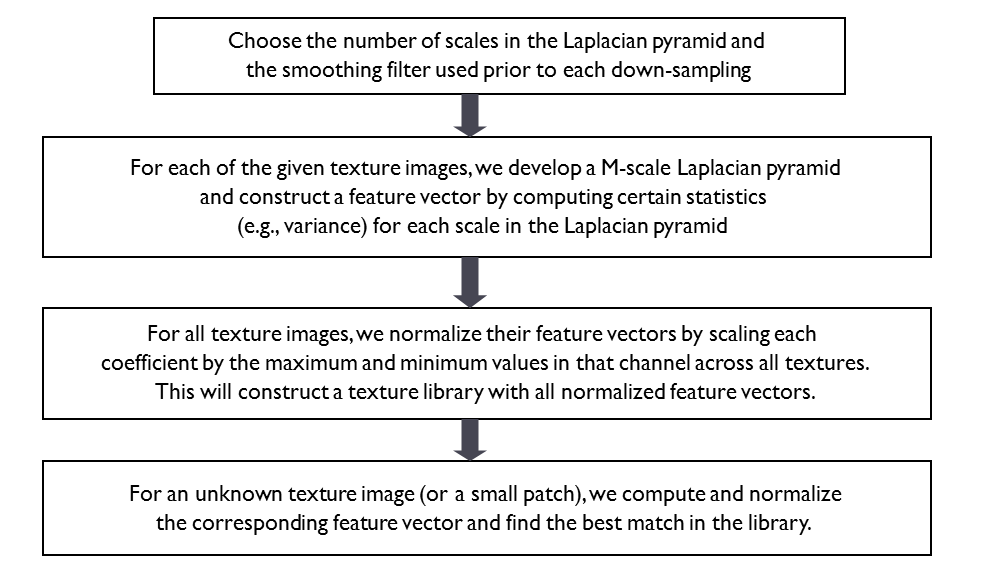
\includegraphics[width=\textwidth]{lap-flow.png}
\end{figure}
\end{frame}

\begin{frame}
\frametitle{Gabor Filter Bank Texture Classification}
\begin{figure}
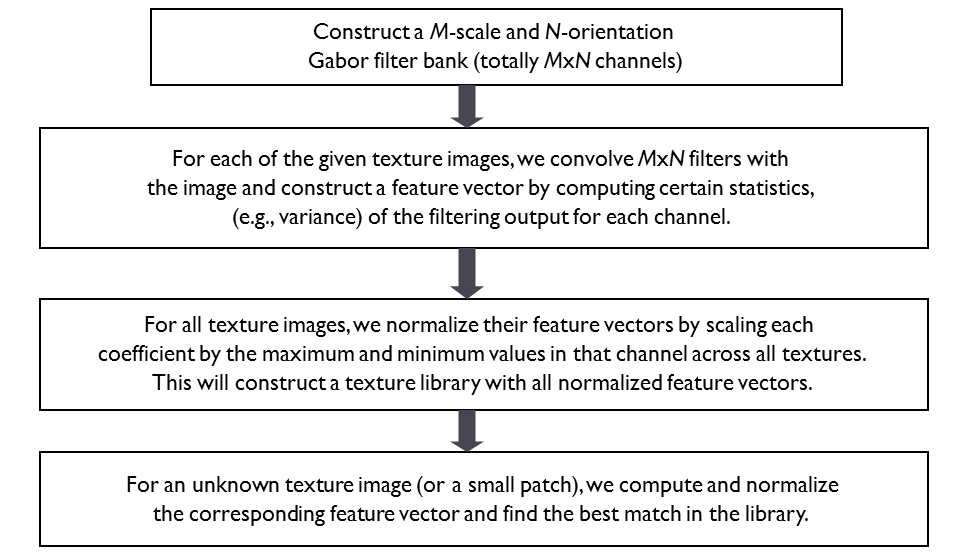
\includegraphics[width=\textwidth]{gabor-flow.png}
\end{figure}
\end{frame}

\begin{frame}
\frametitle{Issues With Texture Classification}
\begin{itemize}
	\item \textbf{Scales:} Mean, variance, skewness, Kurtiosis
	\item \textbf{Size and Orientation:} Kernel window size, orientation and standard deviation 
\end{itemize}

\end{frame}

\begin{frame}
\frametitle{Laplacian Basic Implementation {$67.53\%$}}
\begin{columns}[T] % align columns
\begin{column}{.8\textwidth}
\begin{table}
	\resizebox{.14\linewidth}{!}{
	\pgfplotstabletypeset[%
         col sep=comma,
         header=has colnames,
         columns={Texture Num,PCC},
         columns/Texture Num/.style={string type},
         columns/PCC/.style={dec sep align}, 
	   ]{lapalacian_basic.csv}
	}
	\caption{Projection Matrix M}
\end{table}
\end{column}
\end{columns}
\end{frame}

\begin{frame}
\frametitle{Basic Laplacian Pyramid Building Pitfalls}
\begin{itemize}
	\item Kernels can be smoothed in all layers using same parameters
	\item Distance metric for all the layers are same
	\item All the pixels are convoluted similar way if same variance and window size is used
\end{itemize}
\end{frame}

\begin{frame}
\frametitle{Practical Observation in Laplacian Pyramid}
\begin{itemize}
	\item Laplacian Pyramid is Built by Smoothing and Down Sampling
	\item It does not make sense to use same smoothing parameter for a image which half in size than previous layer
	\item Specifically, smallest layer convoluted with large kernel with small $\sigma$ can make it look like uniform distribution
	\item Pixels nearby boundary are affected by boundary in convolution
	\item Distance Metric in all layer are not the same
\end{itemize}
% \end{frame}

\begin{frame}
\frametitle{Laplacian Pyramid Best AVG PCC {$76.98\%$}}
\begin{columns}[T] % align columns
\begin{column}{.8\textwidth}
\begin{table}
	\resizebox{.14\linewidth}{!}{
	\pgfplotstabletypeset[%
         col sep=comma,
         header=has colnames,
         columns={Texture Num,PCC},
         columns/Texture Num/.style={string type},
         columns/PCC/.style={dec sep align}, 
	   ]{lap_best.csv}
	}
	\caption{Projection Matrix M}
\end{table}
\end{column}
\end{columns}
\end{frame}

\begin{frame}
\frametitle{Laplacian Pyramid Insights: Good Case PCC {$100\%$}}
\begin{figure}
\centering
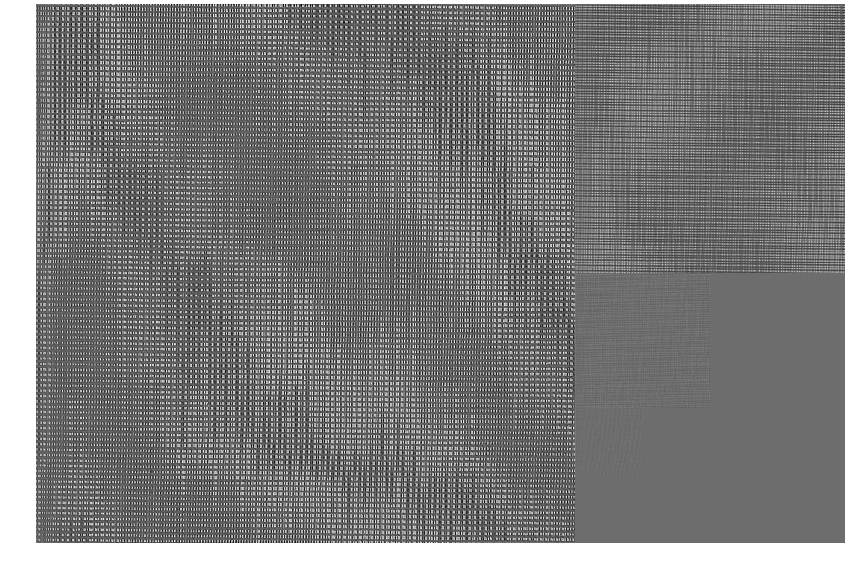
\includegraphics[height=.3\textheight]{lap_good/lib_k_7_sig_0_85_stat_2.png}\vfill
\caption{Laplacian Pyramid Library D21}
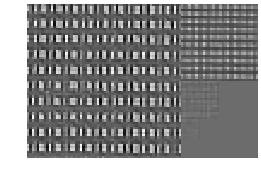
\includegraphics[height=.15\textheight]{lap_good/k_7_sig_0_85_stat_2_blk_56.png}\vfill
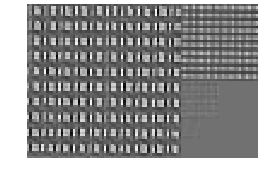
\includegraphics[height=.15\textheight]{lap_good/k_7_sig_0_85_stat_2_blk_100.png}
\caption{Laplacian Pyramid Blocks 56 and 100th blocks}
\end{figure}
\end{frame}

% \begin{frame}
% \frametitle{Laplacian Pyramid Insights: Good Case PCC {$100\%$}}
% \begin{figure}
% \centering
% 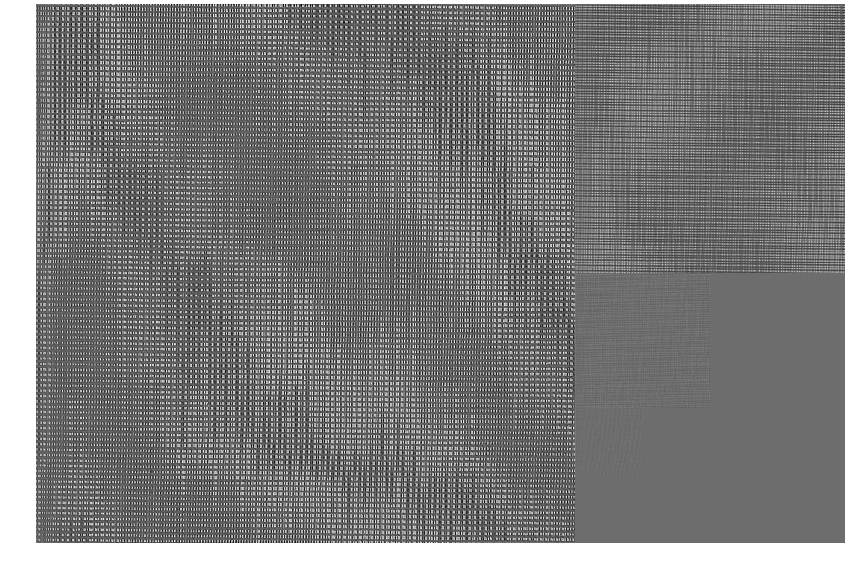
\includegraphics[height=.4\textheight]{lap_good/lib_k_7_sig_0_85_stat_2.png}\vfill
% \caption{Laplacian Pyramid Library}
% 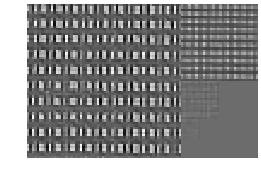
\includegraphics[height=.1\textheight]{lap_good/k_7_sig_0_85_stat_2_blk_56.png}\vfill
% 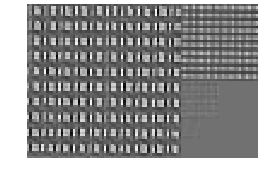
\includegraphics[height=.1\textheight]{lap_good/k_7_sig_0_85_stat_2_blk_100.png}
% \caption{Laplacian Pyramid Blocks 56 and 100th blocks}
% \end{figure}
% \end{frame}

\begin{frame}
\frametitle{Laplacian Pyramid Insights: Bad Case PCC {$28\%$}}
\begin{figure}
\centering
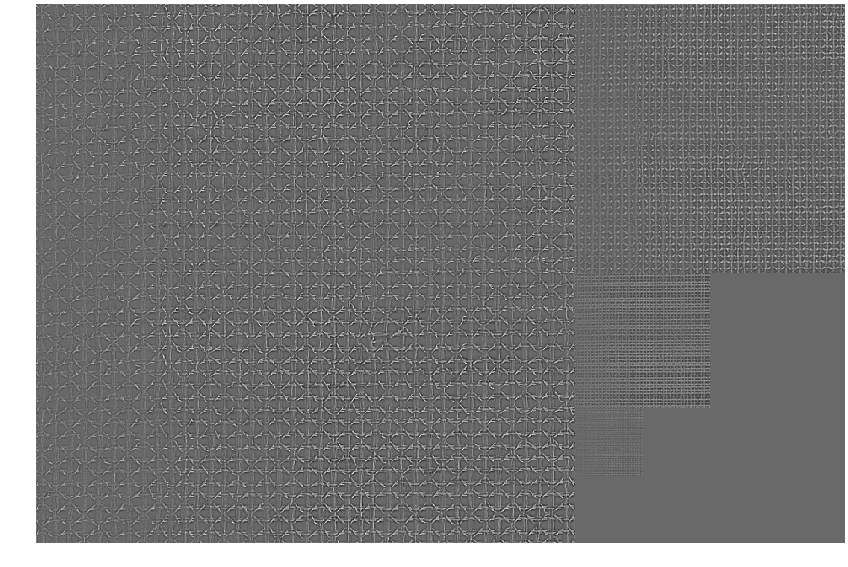
\includegraphics[height=.4\textheight]{lap_bad/lib_k_7_sig_0_85_stat_2.png}\vfill
\caption{Laplacian Pyramid Library D51}
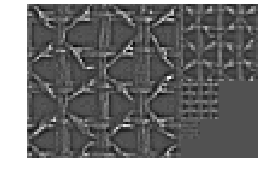
\includegraphics[height=.1\textheight]{lap_bad/k_7_sig_0_85_stat_2_blk_45.png}\vfill
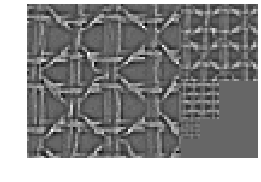
\includegraphics[height=.1\textheight]{lap_bad/k_7_sig_0_85_stat_2_blk_100.png}
\caption{Laplacian Pyramid Blocks 45 and 100th blocks}
\end{figure}
\end{frame}

\begin{frame}
\frametitle{Laplacian Pyramid Optimization}
% Please add the following required packages to your document preamble:
% \usepackage{booktabs}
\begin{table}[]
\centering
\caption{Optimum Kernel Variance Parameter}
\label{my-label}
\begin{tabular}{@{}ll@{}}
\toprule
Window Size & Variance \\ \midrule
8           & .883     \\
16          & .865     \\
32          & .854     \\
64          & .8525    \\
80          & .825     \\
160         & .848     \\
320         & .849     \\
640         & .847     \\ \bottomrule
\end{tabular}
\end{table}
\end{frame}

\begin{frame}
\frametitle{Laplacian Pyramid Optimization}
\begin{itemize}
	\item Mahalonobis distance gave best PCC
	\item Euclidean Distance give $71.3\%$ PCC which was outperformed by Mahalonobis
	\item Variance and Kurtiosis used combinedly for 640 and 320 sized kernel
	\item For 160 and smaller kernel only variance was used
\end{itemize}
\end{frame}

\section{Gabor Filter Texture Classification}
\begin{frame}
\frametitle{Gabor Filter Texture Classification}
\begin{itemize}
	\item 4 Scale and 6 orientation; 24 channels have been used for Gabor Filter Bank
	\item Varian, Kurtiosis and Skewness combinedly were used to build feature vector
	\item Cosine Distance Produced best PCC of $87.58\%$ 
	\item Mahalonobis Euclidean Distance Produced PCC $85.12\%$
\end{itemize}
\end{frame}

\begin{frame}
\frametitle{Log-Gabor Pyramid AVG PCC {$87.58\%$}}
\begin{columns}[T] % align columns
\begin{column}{.8\textwidth}
\begin{table}
	\resizebox{.135\linewidth}{!}{
	\pgfplotstabletypeset[%
         col sep=comma,
         header=has colnames,
         columns={TextureNum,PCC},
         columns/TextureNum/.style={string type},
         columns/PCC/.style={dec sep align}, 
	   ]{gabor_best.csv}
	}
	\caption{Projection Matrix M}
\end{table}
\end{column}
\end{columns}
\end{frame}

\begin{frame}
\frametitle{Log Gabor Kernels and Spread}
\begin{figure}
\centering
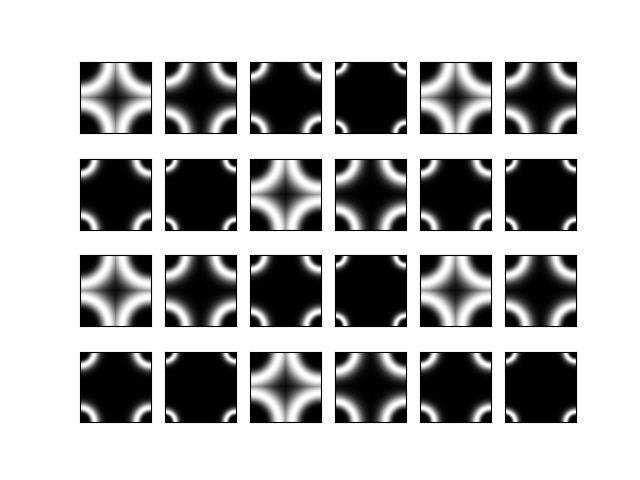
\includegraphics[height=.4\textheight]{loggabor.png}\vfill
\caption{Log Gabor kernel. Gabor kernel has a different signature which was shown in the class but we are using log gabor here}
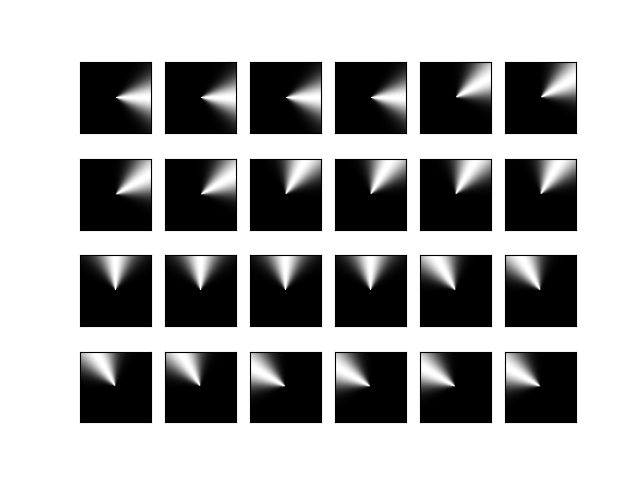
\includegraphics[height=.3\textheight]{spread.png}
\caption{Spread orientation}
\end{figure}
\end{frame}
% ------------------------------------------------------------------------------------------------------------------

\section{Conclusion}
\begin{frame}
\frametitle{Conclusion}
\begin{columns}
\column{\textwidth}
\centering
\begin{itemize}
\item \textbf{Thank You}
\item \textbf{Questions ?}
\end{itemize}
\end{columns}
\end{frame}

% ------------------------------------------------------------------------------------------------------------------

\end{document}

